\chapter{O projeto do arranjo físico (\textit{Lay-out})}
\label{chap:projeto_do_arranjo}
O arranjo físico (\textit{lay-out}) dos equipamentos é a disposição que os equipamentos possuem na fábrica, de modo que proporcionem a máxima eficiência dentro do processo produtivo.

Os principais tipos de arranjos físicos são o Posicional ou Fixo, arranjo em que os equipamentos e operadores movem-se durante as operações; Físico por Processo, onde os equipamentos possuem posicionamento fixo; Físico Celular ou Células de Produção, onde os materiais fluem somente através de suas células específicas e o arranjo Físico por Produto (em linha), onde os materiais fluem através de equipamentos fixos, por um único e exclusivo roteiro, do início ao fim do processamento.

Antes de escolher o \textit{lay-out} é importante que se considere todo o fluxo do processo da produção. Cada tipo de processo produtivo se encaixa em um dos quatro modelos mais comuns de arranjos físicos. Quantidade do produto a ser produzido, variedade de produtos que serão produzidos e o tipo de produto a ser produzido são os principais fatores a serem considerados antes da escolha do \textit{lay-out} de produção.

Compreender o fluxo de trabalho da fábrica, o tipo de elemento a ser produzido, suas especificações e volume são fatores determinantes na escolha do \textit{lay-out} de produção. É também primordial posicionar os postos de trabalho próximos as máquinas para economizar tempo de percurso, mesmo mantendo o espaço reservado às áreas de segurança.

\section{Aplicação Prática}
\label{sec:projeto_do_arranjo_aplicacao}
A SunBurn possui o arranjo físico descrito na Figura \ref{fig:arranjo_fisico_aplicacao} onde é possível identificar que a planta de energia solar é dividida em duas subplantas, 1 e 2, e há uma subestação, que recebe a energia gerada pelas placas fotovoltaicas e é responsável por converter corrente contínua (das placas) em corrente alternada, e enviar a energia para a cliente, Chesf.


\begin{figure}[H]
    \caption{Layout da planta de energia solar da SunBurn.} 
    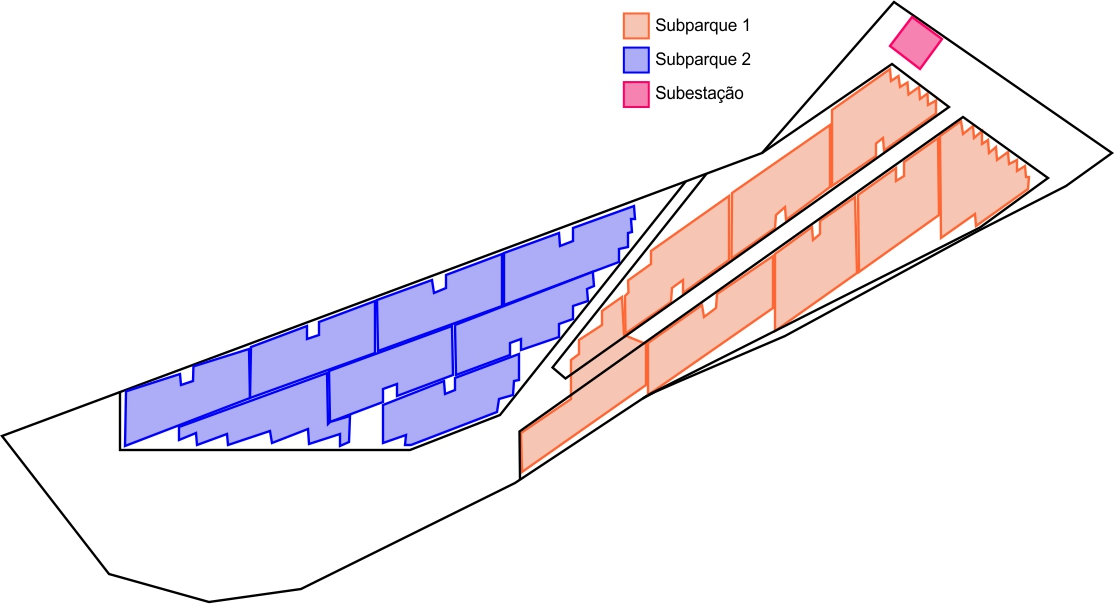
\includegraphics[width=1\textwidth]{images/layout.jpg}
    \caption*{Fonte: modificado SunBurn.}
    \label{fig:arranjo_fisico_aplicacao}
  \end{figure}